\documentclass[12pt,a4paper]{article}

% ── Packages ──────────────────────────────────────────────────────────────────
\usepackage[T1]{fontenc}
\usepackage[utf8]{inputenc}
\usepackage[english]{babel}
\usepackage{booktabs}
\usepackage{float}
\usepackage{pgfplots}
\pgfplotsset{compat=1.18}
\usepackage{amsmath}
\usepackage{amssymb}
\usepackage{geometry}
\geometry{margin=2.5cm}
\usepackage{hyperref}
\hypersetup{colorlinks=true, linkcolor=blue, urlcolor=blue}
\usepackage{listings}
\usepackage{xcolor}
\usepackage[protrusion=false,expansion=false]{microtype}
\usepackage{parskip}
\setlength{\parskip}{6pt}
\usepackage{tikz}
\usetikzlibrary{arrows.meta, fit, positioning, shapes.geometric,
                decorations.pathreplacing, calc}

\lstset{
  basicstyle=\ttfamily\small,
  backgroundcolor=\color{gray!8},
  frame=single,
  breaklines=true,
  keywordstyle=\color{blue!70}\bfseries,
  commentstyle=\color{green!50!black},
  numbers=left,
  numberstyle=\tiny\color{gray},
  xleftmargin=1.5em,
}

% ── Title ─────────────────────────────────────────────────────────────────────
\title{
  \textbf{Parallel Ensemble Inference Engine}\\[4pt]
  \large Hybrid MPI + OpenMP Parallelization of a\\ Soft-Voting Classifier\\[8pt]
  \normalsize HPC Project Report,  University of Messina
}
\author{Andrea Fascì}
\date{2025-2026\\[4pt]
\small\url{https://github.com/andre1012345/HPC-inference}}

% ─────────────────────────────────────────────────────────────────────────────
\begin{document}
\maketitle

\begin{abstract}
\emergencystretch=2em
This report presents the design and experimental evaluation of a hybrid
MPI + OpenMP parallel inference engine for a three-model soft-voting
ensemble classifier (K-Nearest Neighbours, Gaussian Naive Bayes, and
Logistic Regression). The ensemble is trained offline (once, in Python, before any inference run;
parameters are then fixed in files and never updated at inference time) on a
fully synthetic binary classification dataset (70{,}000 samples, 20 features)
and achieves 88.44\% accuracy.
At inference time, the test set is distributed across MPI
ranks via \texttt{MPI\_Scatter}; each rank parallelizes its local work with
OpenMP; results are gathered with non-blocking \texttt{MPI\_Isend}/\allowbreak\texttt{MPI\_Irecv}
and accuracy is validated with \texttt{MPI\_Reduce}.
Following Flynn's taxonomy the system is \textbf{MIMD} (Multiple Instruction,
Multiple Data): each active core executes its own instruction stream on its
own data slice independently.
Experiments on an Intel
Core i5\-8350U (4 physical cores, WSL2) show a best speedup of $3.81\times$
at $p=4$ ranks and $t=2$ threads per rank. Scaling is ultimately memory-bound:
each MPI rank independently holds the full 50{,}000 sample training set
($\sim$8\,MB), exceeding the 6\,MB L3 cache and forcing concurrent DRAM
accesses that erode efficiency at higher parallelism levels.
\end{abstract}

\tableofcontents
\newpage

% ─────────────────────────────────────────────────────────────────────────────
\section{Introduction}
% ─────────────────────────────────────────────────────────────────────────────

\subsection{Context}

Batch inference --- classifying a large set of unlabelled samples against a
pre-trained model --- is a routine workload in production machine-learning
pipelines. A \textbf{query} is a single prediction request: one feature vector
$\mathbf{x}$ presented to the model, which returns a predicted class label.
The model is \textbf{trained offline}: parameters are learned once, in a
separate training step, and remain fixed for the lifetime of the inference
engine. No learning occurs at inference time; the engine only reads the
pre-computed parameters and evaluates them.

When one of the models is a brute-force K-Nearest Neighbours
classifier, the cost is $O(N_\text{train} \times F)$ per query: every test
sample must be compared against all training points across all features.
At the scale used here --- 20{,}000 queries against 50{,}000 training points
with 20 features --- this amounts to roughly $4 \times 10^{10}$ floating-point
operations (40~FLOP per training point $\times$ 50{,}000 points $\times$
20{,}000 queries), making sequential execution too slow for any interactive
use case (baseline wall time: $\approx$20.6~s on a four-core laptop).

The problem is a target for data-parallel acceleration: each test
sample is fully independent, so the work can be distributed across workers
without any inter-query communication during inference.
The question addressed in this project is \emph{how} to structure that
parallelism across the two programming models available on a
multi-core machine: MPI for inter-process distribution and OpenMP for
intra-process threading.

\subsection{The Ensemble}

Three classifiers are combined into a soft-voting ensemble:

\begin{itemize}
  \item \textbf{KNN (K-Nearest Neighbours):} stores all 50{,}000 training
        points and computes brute-force distances at query time.
        This is the \emph{dominant cost}: about 86\% of total runtime
        (measured by \texttt{gprof} at \texttt{-O0}; qualitative indicator only).
        Classification accuracy of the algorithm alone: 93.25\%.
  \item \textbf{Naive Bayes (NB):} uses precomputed class means and variances.
        Each prediction is a few arithmetic operations (essentially free).
        Classification accuracy of the algorithm alone: 79.64\%.
  \item \textbf{Logistic Regression (LR):} a dot product plus a sigmoid.
        Also negligible in cost.
        Classification accuracy of the algorithm alone: 80.50\%.
\end{itemize}

Soft voting requires each model to output a \emph{probability}
$P(y{=}1 \mid \mathbf{x}) \in [0,1]$, not just a hard predicted class.
A hard-voting scheme would discard confidence information: a model that
says ``class 1 with 51\% probability'' and one that says ``class 1 with
99\% probability'' would contribute identical votes, even though the
second is far more certain. By averaging continuous probabilities, the
ensemble weights predictions by their implicit confidence.

Each model outputs a probability $P(y{=}1 \mid \mathbf{x})$. The ensemble
combines them by simple average:
\[
  P_\text{ens}(\mathbf{x}) = \frac{P_\text{KNN}(\mathbf{x}) +
                                    P_\text{NB}(\mathbf{x}) +
                                    P_\text{LR}(\mathbf{x})}{3},
  \qquad
  \hat{y} = \begin{cases} 1 & P_\text{ens} \geq 0.5 \\ 0 & \text{otherwise.}
             \end{cases}
\]
Combining the three models gives \textbf{88.44\%} accuracy, above NB and LR
but below KNN alone (93.25\%). The ensemble falls short of KNN because
soft-voting uses equal weights: on samples where KNN predicts correctly but
NB and LR both disagree, the two weaker models can pull
$P_\text{ens}$ across the 0.5 threshold and override KNN's prediction.
The gain over NB and LR nevertheless justifies the ensemble as a more
robust classifier than either lightweight model alone.

\textbf{Why this ensemble design and not boosting or bagging?}
Boosting and bagging improve a \emph{single} base learner; here the three
models have fundamentally different inductive biases (local geometry,
feature independence, linear boundary), so combining them provides
complementary diversity that re-sampling a single learner cannot achieve.

\subsection{Why Parallelize?}

KNN dominates the computational budget. Here $N_\text{train} = 50{,}000$
is the number of training points, $F = 20$ the number of features, and
$C = 2$ the number of classes. Each test query requires a full scan of the
training set, one squared-distance computation per training point,
followed by a \texttt{partial\_sort} to extract the $k$ nearest neighbours.
The per-query cost is $O(N_\text{train} \times F)$, giving a total of:
%
\[
  20{,}000 \times 50{,}000 \times 40 \approx 4 \times 10^{10}
  \text{ floating-point operations (40\,FLOP per training-point comparison)}
\]
%
LR and NB contribute $O(F)$ and $O(C \times F)$ per query respectively, four to five orders of magnitude
less, and are effectively free by comparison.

Critically, test queries are mutually independent: the prediction for sample
$i$ depends only on \texttt{X\_train} and the model parameters, not on any
other test sample. This structure means the workload
can be partitioned across processes and threads with zero inter-query
synchronization, making parallelization both natural and efficient.

\subsection{Proposed Solution}

The hybrid binary \texttt{inference\_dist\_knn.cpp} partitions the inference
workload across two levels of parallelism:

\begin{enumerate}
  \item \textbf{MPI\_Scatter} distributes the test set evenly across $p$
        ranks; each rank receives $N_\text{test}/p$ samples and holds a
        full copy of \texttt{X\_train}, preserving exact KNN accuracy.
  \item \textbf{OpenMP} parallelises the per-sample inference loop inside
        each rank with a single \texttt{parallel for} (schedule static),
        one fork/join per timed run rather than per sample.
  \item \textbf{MPI\_Isend/MPI\_Irecv + MPI\_Waitall} gather local
        predictions at rank~0 non-blockingly; rank~0 posts all receives
        simultaneously so multiple in-flight transfers proceed concurrently
        rather than sequentially.
  \item \textbf{MPI\_Reduce} aggregates per-rank correct-prediction counts
        for a single global accuracy figure.
\end{enumerate}

The two-level design has a concrete memory implication: each MPI rank holds
one independent copy of \texttt{X\_train}. On the test machine ($p \leq 4$),
this means at most four 8\,MB copies in DRAM simultaneously, a deliberate
trade-off between memory footprint and the complexity of distributing the
training set across ranks, which would require approximate rather than exact
KNN.

\subsection{The Hybrid Parallelism Hierarchy}
\label{sec:hybrid}

The two programming models are not interchangeable: they operate at
different granularities and carry fundamentally different memory semantics.
Crucially, OpenMP is \emph{confined to a single node}: threads share
one address space and therefore one physical host. MPI processes have
independent address spaces and communicate over a network, so they are
the only mechanism that can distribute work across multiple nodes in a
cluster. A pure-OpenMP design would be limited to the cores on one
machine; the hybrid design retains that option while opening the door
to multi-node scaling.

According to Flynn's taxonomy, this architecture is \textbf{MIMD} (Multiple
Instruction, Multiple Data): every active core executes its own instruction
stream on its own data slice, independently of all others. This is the
defining property of both MPI processes (each running a separate OS process)
and OpenMP threads (each executing the loop body on a distinct iteration).
SIMD would apply if a single instruction simultaneously operated on multiple
data lanes (e.g.\ AVX vector units); that is a separate micro-architectural
feature orthogonal to the parallel programming models used here.

MPI parallelism is \emph{coarse-grained}. Each rank is an independent OS
process with its own address space; inter-rank communication requires
explicit messaging. This makes MPI robust against false sharing and
cache-coherence traffic, but each rank must hold its own copy of
\texttt{X\_train}. Scaling MPI ranks alone multiplies memory pressure
proportionally.

OpenMP parallelism is \emph{fine-grained}. Threads within a rank share the
same address space, so \texttt{X\_train} and the model parameters are loaded
once and read concurrently without copying. The cost is potential contention
on shared data structures --- avoided here because each thread writes to a
disjoint index of \texttt{local\_preds[i]} and uses pre-allocated private
buffers (\texttt{dist\_bufs[tid]}, \texttt{idx\_bufs[tid]}).

The hybrid design exploits both properties simultaneously: MPI distributes
the test set across $p$ processes (reducing per-rank work), while OpenMP
extracts parallelism within each process without multiplying the memory
footprint. The total worker count is $p \times t$;
Figure~\ref{fig:hybrid_hierarchy} illustrates this for $p=2$, $t=2$.

\begin{figure}[H]
\centering
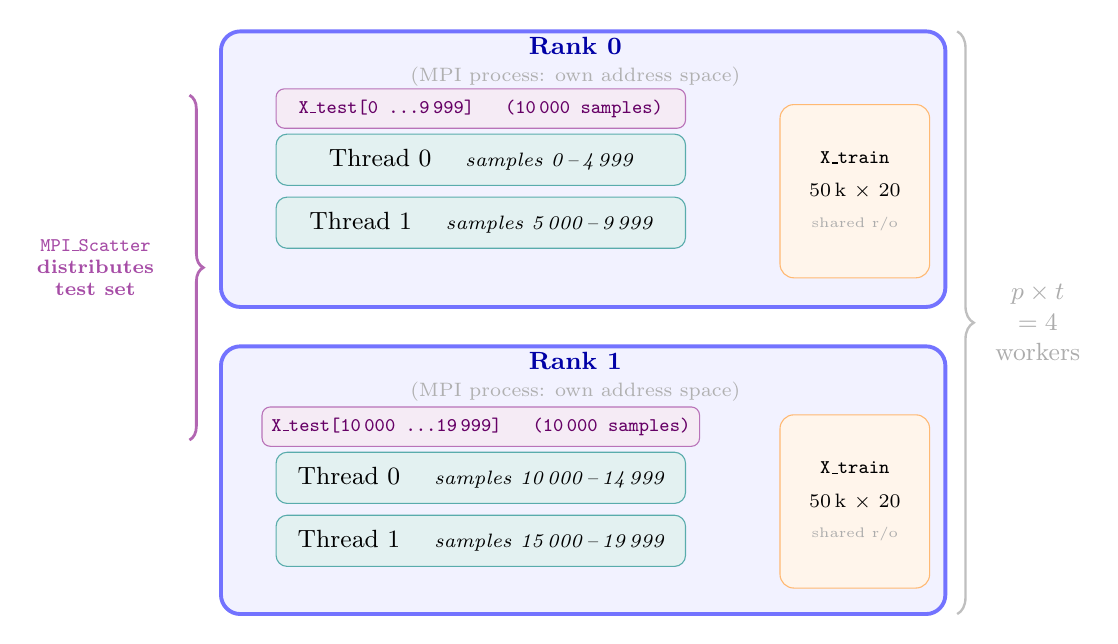
\begin{tikzpicture}[
  rankbox/.style  = {draw=blue!55,   fill=blue!5,    rounded corners=7pt,
                     line width=1.4pt},
  tbox/.style     = {draw=teal!65,   fill=teal!11,   rounded corners=4pt,
                     minimum width=5.2cm, minimum height=0.65cm, font=\small},
  datarow/.style  = {draw=violet!55, fill=violet!8,  rounded corners=3pt,
                     minimum width=5.2cm, minimum height=0.50cm,
                     font=\scriptsize\ttfamily, text=violet!80!black},
  trainbox/.style = {draw=orange!55, fill=orange!8,  rounded corners=5pt,
                     font=\scriptsize, align=center,
                     minimum width=1.9cm, minimum height=2.2cm},
  head/.style     = {font=\small\bfseries, blue!65!black},
  sublbl/.style   = {font=\scriptsize, gray!62},
]

%% ── Rank 0 ──────────────────────────────────────────────────────────────────
\draw[rankbox] (-3.2, 1.0) rectangle (6.0, 4.5);
\node[head]   at (1.3, 4.32) {Rank 0};
\node[sublbl] at (1.3, 3.92) {(MPI process: own address space)};

\node[datarow] at (0.1, 3.52)
  {\texttt{X\_test[0 \ldots 9\,999]} \quad (10\,000 samples)};

\node[tbox] at (0.1, 2.87)
  {Thread 0 \quad {\scriptsize\itshape samples 0\,--\,4\,999}};
\node[tbox] at (0.1, 2.07)
  {Thread 1 \quad {\scriptsize\itshape samples 5\,000\,--\,9\,999}};

\node[trainbox] at (4.85, 2.47)
  {\texttt{X\_train}\\[4pt]50\,k $\times$ 20\\[3pt]\textcolor{gray!65}{\tiny shared r/o}};

%% ── Rank 1 ──────────────────────────────────────────────────────────────────
\draw[rankbox] (-3.2,-2.9) rectangle (6.0, 0.5);
\node[head]   at (1.3, 0.32) {Rank 1};
\node[sublbl] at (1.3,-0.08) {(MPI process: own address space)};

\node[datarow] at (0.1,-0.52)
  {\texttt{X\_test[10\,000 \ldots 19\,999]} \quad (10\,000 samples)};

\node[tbox] at (0.1,-1.17)
  {Thread 0 \quad {\scriptsize\itshape samples 10\,000\,--\,14\,999}};
\node[tbox] at (0.1,-1.97)
  {Thread 1 \quad {\scriptsize\itshape samples 15\,000\,--\,19\,999}};

\node[trainbox] at (4.85,-1.47)
  {\texttt{X\_train}\\[4pt]50\,k $\times$ 20\\[3pt]\textcolor{gray!65}{\tiny shared r/o}};

%% ── MPI\_Scatter brace on left ───────────────────────────────────────────────
\draw[decorate, decoration={brace, amplitude=5pt},
      violet!60, line width=1.0pt]
  (-3.6, 3.69) -- (-3.6,-0.69)
  node[midway, left=9pt, font=\scriptsize\bfseries, violet!70, align=center]
  {\texttt{MPI\_Scatter}\\distributes\\test set};

%% ── p×t brace on right ───────────────────────────────────────────────────────
\draw[decorate, decoration={brace, amplitude=6pt, mirror},
      gray!50, line width=0.85pt]
  (6.15,-2.9) -- (6.15, 4.5)
  node[midway, right=10pt, font=\small, gray!65, align=center]
  {$p \times t$\\$= 4$\\workers};

\end{tikzpicture}
\caption{The two-level hybrid hierarchy for $p=2$, $t=2$.
  The violet strip inside each rank shows the \texttt{X\_test} slice delivered
  by \texttt{MPI\_Scatter}; OpenMP then subdivides that slice among threads
  (sample ranges shown). Each rank independently holds a full copy of
  \texttt{X\_train} (shared read-only among its threads).}
\label{fig:hybrid_hierarchy}
\end{figure}

% ─────────────────────────────────────────────────────────────────────────────
\section{Problem Rationale}
% ─────────────────────────────────────────────────────────────────────────────

The parallel design follows a deliberate three-step workflow: (1)~train the
ensemble offline once in Python to produce fixed model-parameter files;
(2)~implement and profile a sequential C++ baseline to identify the
computational hotspot; (3)~build the hybrid engine targeting that hotspot.
This section documents steps~1 and~2. The parallel design is formalised
in Sections~\ref{sec:decomposition}--\ref{sec:mapping}.

\subsection{Problem Statement}

\textbf{Input:} a pre-trained ensemble (KNN, NB, LR) and a test set of
20{,}000 samples with 20 features each.\\
\textbf{Output:} one binary prediction per sample, matching the accuracy of
the sequential implementation.\\
\textbf{Goal:} minimize wall-clock time on a multi-core machine.

\subsection{Dataset}

The dataset is \textbf{fully synthetic}, generated with scikit-learn via
\texttt{train.py}:

\begin{lstlisting}[language=Python]
X, y = make_classification(
    n_samples=70_000, n_features=20,
    n_informative=10, n_redundant=2,
    n_classes=2, class_sep=1.0, random_state=42
)
\end{lstlisting}

The 70{,}000 samples are split 50{,}000 / 20{,}000 (train / test) with
stratified sampling. Features are standardised with a \texttt{StandardScaler}
fitted on training data only; this step is critical for KNN because Euclidean
distance is sensitive to feature scale---without normalisation a feature with a
large numerical range would dominate the distance calculation and suppress the
remaining 19 features. The script trains all three models and exports all parameters as plain-text
files to \texttt{model\_params/}: the full $50{,}000\times20$ training
matrix (\texttt{X\_train.txt}) and labels (\texttt{y\_train.txt}) for KNN;
per-class per-feature means (\texttt{nb\_means.txt}) and variances
(\texttt{nb\_vars.txt}) plus class priors (\texttt{nb\_priors.txt}) for NB;
and a weight vector (\texttt{lr\_weights.txt}) with a scalar bias
(\texttt{lr\_bias.txt}) for LR. The C++ engine loads these files at
startup and performs no training; the Python script is never called at
inference time.

A synthetic dataset was chosen for full reproducibility and to avoid any
licensing or data-provenance issues.

\subsection{Sequential Solution}
\label{sec:sequential}

The sequential binary (\texttt{inference\_seq.cpp}) serves two purposes:
it is the \textbf{profiling target} that reveals which operation dominates
runtime (Section~\ref{sec:profiling}), and it provides the reference
wall-clock time $T_1$ against which all parallel speedups are measured
(Section~\ref{sec:perf}). It processes one test sample at a time:

\begin{enumerate}
  \item \textbf{KNN inference} (\texttt{knn\_distances\_tiled} + \texttt{partial\_sort}):
        iterates over all 50{,}000 training
        points, computes squared Euclidean distances via the tiled kernel, runs
        \texttt{partial\_sort} to find the $k=5$ nearest neighbours, then
        returns $P(y{=}1 \mid \mathbf{x}) = c_1 / k$ where $c_1$ is the
        number of neighbours whose label is 1 (e.g.\ 3 class-1 neighbours
        $\Rightarrow P = 3/5 = 0.60$).
        \texttt{partial\_sort} is preferred over a full sort because it runs
        in $O(n \log k)$ time rather than $O(n \log n)$: only the $k=5$
        smallest distances need to be ordered, so the algorithm stops as
        soon as the $k$-th element is placed correctly. With $n = 50{,}000$
        and $k = 5$ this gives roughly a $4\times$ saving in the sort phase.
  \item \texttt{nb\_predict\_proba}: computes the Gaussian log-posterior
        for each class $c \in \{0,1\}$ using the precomputed per-class,
        per-feature means $\mu_{c,j}$ and variances $\sigma^2_{c,j}$:
        \[
          \log P(y{=}c \mid \mathbf{x}) = \log P(c)
            + \sum_{j=1}^{F}
              \left[
                -\tfrac{1}{2}\log(2\pi\sigma^2_{c,j})
                - \frac{(x_j - \mu_{c,j})^2}{2\sigma^2_{c,j}}
              \right]
        \]
        Log-sum-exp normalisation converts the two raw log-posteriors to
        probabilities that sum to 1.
  \item \texttt{lr\_predict\_proba}: $\sigma(\mathbf{w} \cdot \mathbf{x} + b)$.
\end{enumerate}

The KNN distance and index scratch buffers (50{,}000 elements each) are
allocated \emph{once} before the run loop and reused across all samples.
The binary is compiled with \texttt{-O2} and benchmarked under the same
cold-cache conditions as all parallel configurations.

\subsection{Profiling}
\label{sec:profiling}

The sequential binary was compiled with \texttt{-O0 -pg} and profiled with
\texttt{gprof} to find the hotspot. Table~\ref{tab:gprof} shows the result.

\begin{table}[H]
  \centering
  \caption{\texttt{gprof} flat profile top entries (compiled \texttt{-O0 -pg},
           sequential baseline, $N\_RUNS=3$).
           \texttt{knn\_distances\_tiled} is called 15{,}000 times
           $= 3\ \text{runs} \times 5{,}000\ \text{batches}$
           (\texttt{TILE\_Q}=4, so $20{,}000 / 4$ batches per run).
           The iterator-infrastructure entries
           (\texttt{\_\_fill\_a1}, lambda comparators, etc.)\ are \texttt{-O0}
           instrumentation artefacts; at \texttt{-O2} they inline into the
           distance kernel and sort, leaving no separate symbol.
           Absolute times are not meaningful at \texttt{-O0}; only the
           relative hotspot breakdown is indicative.
           NB and LR together account for 0.01\% --- effectively free.}
  \label{tab:gprof}
  \begin{tabular}{rll}
    \toprule
    \textbf{\% time} & \textbf{Function} & \textbf{Calls} \\
    \midrule
    86.28 & \texttt{knn\_distances\_tiled} (tiled distance kernel) & 15{,}000 \\
     2.79 & \texttt{std::iota} (index reset per query)             & 60{,}000 \\
     1.70 & \texttt{std::\_\_heap\_select} (\texttt{partial\_sort} core) & 60{,}000 \\
    $\approx$9 & iterator/buffer internals (\texttt{-O0} artefact, inlined at \texttt{-O2}) & --- \\
     0.01 & \texttt{nb\_predict\_proba}                            & 60{,}000 \\
     0.00 & \texttt{lr\_predict\_proba}                            & 60{,}000 \\
    \bottomrule
  \end{tabular}
\end{table}

\noindent
NB and LR together account for approximately 0.01\% of runtime --- effectively free.
All parallelization effort is therefore correctly directed at the outer loop
over test samples, where \texttt{knn\_distances\_tiled} is called.

The binary was compiled with \texttt{-O0} to prevent the compiler from
inlining or collapsing call chains, keeping individual functions visible
to the sampler. The absolute times carry no performance significance;
the profile is used solely to confirm the hotspot. All benchmarks in
Section~\ref{sec:perf} use \texttt{-O2}.

This finding drives the entire parallel design: \texttt{knn\_distances\_tiled}
dominates runtime and each test sample is independent, so decomposing the
test set across workers and parallelising the outer sample loop is the
correct strategy. The PCAM decomposition in
Section~\ref{sec:decomposition} formalises this choice.

\subsection{Existing Parallel Approaches}

Three strategies are commonly used to parallelise brute-force KNN inference;
the choice between them has direct consequences for communication overhead
and accuracy.

\textbf{Test-set decomposition} assigns each worker a disjoint slice of the
test set while every worker retains the full training set. No inter-worker
communication occurs during the inference loop; a single scatter before and
a single gather after are sufficient. Giacomazzi et al.~\cite{giacomazzi2006}
demonstrate that a three-level hierarchy of threads, MPI processes, and Grid
nodes built on this decomposition achieves speedups exceeding $15\times$ for
large-scale epidemiological classification workloads. This is the strategy
adopted in this project.

\textbf{Training-set decomposition} partitions \texttt{X\_train} across
workers; each computes partial distances, and a reduce step merges the global
$k$ nearest neighbours before classification. This eliminates the per-rank
copy of training data but introduces communication on the critical path of
every query. Ignatij~\cite{ignatij2022} implements both strategies with MPI
and reports that test-set decomposition consistently outperforms training-set
decomposition, motivating the choice made here.

\textbf{Approximate KNN} replaces exact search with index structures ---
trees, graphs, or quantization, reducing per-query cost from
$O(N_\text{train})$ to $O(\log N_\text{train})$ at the cost of recall.
Johnson et al.~\cite{johnson2017faiss} show that FAISS scales to
billion-scale datasets with controllable accuracy loss. For this project,
however, exact reproducibility of the sequential accuracy (88.44\% across
all configurations) was a hard requirement, which excludes approximate
methods by definition.

% ─────────────────────────────────────────────────────────────────────────────
\section{Decomposition and Partitioning}
\label{sec:decomposition}
% ─────────────────────────────────────────────────────────────────────────────

The design follows Foster's PCAM methodology (Partition, Communicate,
Agglomerate, Map).

\subsection{Partitioning}

A \textbf{hybrid decomposition} strategy is applied at two levels, each
following data (domain) decomposition, mirroring the parallelism hierarchy
of Section~\ref{sec:hybrid}. Hybrid decomposition is appropriate here
because the two levels operate at different granularities and carry different
memory semantics: the MPI level is coarse-grained with independent address
spaces, the OpenMP level is fine-grained with shared memory. The decomposition
strategy is not recursive (no divide-and-conquer splitting) and not
exploratory (every sample must be evaluated; no search space is pruned).

\textbf{MPI level (coarse).}
The 20{,}000 samples are split into $p$ equal chunks, one per MPI rank.
Each chunk is independent: the inference for sample $i$ depends only on
$\mathbf{x}_i$ and the shared read-only model parameters. The MPI level
controls the coarse dependency boundary: \texttt{MPI\_Scatter} must
complete before inference begins, and inference must complete before
\texttt{MPI\_Isend}/\texttt{MPI\_Irecv} gather the results.

\textbf{OpenMP level (fine).}
Within each rank, the $N_\text{test}/p$ local samples are further subdivided
among $t$ threads by the \texttt{schedule(static)} clause, which assigns
contiguous blocks. Contiguous assignment preserves spatial locality: each
thread steps through its slice of \texttt{X\_test\_local} in order, keeping
hardware prefetch streams intact. \texttt{schedule(dynamic)} would interleave
accesses across threads and break the sequential stride. The OpenMP level
controls the fine dependency boundary: the implicit barrier at the end of
the parallel region ensures all threads finish before the rank proceeds to
communication.

When $p$ does not divide 20{,}000 evenly (e.g.\ $p=3$), the test set is
trimmed to the nearest multiple of $p$ before scattering; at $p=3$ this drops
2 samples (19{,}998 classified), a loss of 0.01\% that does not affect the
accuracy comparison.

This gives up to 20{,}000 tasks, three to four orders of magnitude larger
than the maximum process count tested ($p=4$), which satisfies Foster's
requirement.

Functional decomposition (one model per rank) was considered but rejected:
since KNN completely dominates, splitting the models would leave non-KNN ranks
idle almost all the time.

\subsection{Task Dependency Graph (TDG)}

The TDG models the computational structure of the problem in terms of
tasks and their logical dependencies, independently of any implementation
technology. MPI ranks and OpenMP threads are not visible here; they appear
later in the Mapping phase.

\textbf{Algorithm-level structure.}
The inference problem decomposes into $N$ independent \emph{sample groups}.
Each group $i$ contains three mutually independent compute tasks
(KNN$_i$, NB$_i$, LR$_i$) that all read the same $\mathbf{x}_i$ and feed
a per-sample vote task (Vote$_i$). All $N$ vote results feed a single
Aggregate task which computes global accuracy.

Two structural properties are immediately visible from the graph:

\begin{enumerate}
  \item \textbf{No inter-sample dependencies.} Sample group $i$ and group
        $j$ share no data flow. The $N$ groups can execute in any order or
        simultaneously. This is
        the property that the domain decomposition exploits directly.
  \item \textbf{Single global synchronisation point.} Aggregate is the only
        node that depends on the entire computation. It cannot begin until
        all $N$ Vote tasks complete, making it the irreducible serial
        fraction. The profiler attributes $\approx 0.01\%$ to NB and LR combined;
        I/O and communication fall below the sampling threshold.
        Section~\ref{sec:perf} derives the effective serial fraction from
        measured speedups once memory-bandwidth contention is accounted for.
\end{enumerate}

\textbf{Critical path.}
Since all sample groups have identical cost (each KNN task searches the
same 50{,}000 training points), every root-to-leaf path in the TDG has
equal length. The critical path is therefore:
\[
  \text{KNN}_i \;\longrightarrow\; \text{Vote}_i \;\longrightarrow\;
  \text{Aggregate}
\]
for any $i$. Its length sets the minimum achievable parallel execution time
regardless of how many processors are available.

\begin{figure}[H]
\centering
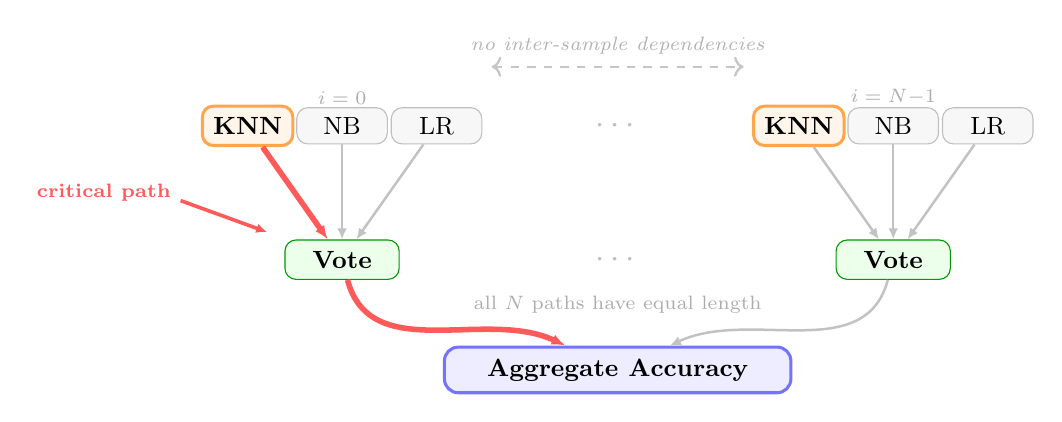
\begin{tikzpicture}[
  knnnode/.style = {draw=orange!70, fill=orange!8, rounded corners=4pt,
                    minimum width=1.15cm, minimum height=0.50cm,
                    font=\small\bfseries, line width=1.1pt},
  mnode/.style   = {draw=gray!50,   fill=gray!6,    rounded corners=4pt,
                    minimum width=1.15cm, minimum height=0.46cm, font=\small},
  votenode/.style= {draw=green!60!black, fill=green!8, rounded corners=4pt,
                    minimum width=1.45cm, minimum height=0.50cm,
                    font=\small\bfseries},
  aggnode/.style = {draw=blue!55, fill=blue!7, rounded corners=5pt,
                    minimum width=4.4cm, minimum height=0.58cm,
                    font=\small\bfseries, line width=1.1pt},
  cparr/.style   = {-{Latex[length=5pt,width=4pt]}, line width=2.0pt, red!65},
  garr/.style    = {-{Latex[length=4pt,width=3.5pt]}, line width=0.9pt, gray!48},
  lbl/.style     = {font=\scriptsize, gray!65},
]

%% ── Sample group i=0 ──────────────────────────────────────────────
\node[knnnode] (knn0) at (-4.7, 2.8) {KNN};
\node[mnode]   (nb0)  at (-3.5, 2.8) {NB};
\node[mnode]   (lr0)  at (-2.3, 2.8) {LR};
\node[votenode](v0)   at (-3.5, 1.1) {Vote};
\draw[cparr] (knn0) -- (v0);
\draw[garr]  (nb0)  -- (v0);
\draw[garr]  (lr0)  -- (v0);
\node[lbl, above=4pt] at (-3.5, 2.8) {$i = 0$};

%% ── Dots ──────────────────────────────────────────────────────────
\node[font=\large, gray!50] at (0, 2.8) {$\cdots$};
\node[font=\large, gray!50] at (0, 1.1) {$\cdots$};

%% ── Sample group i=N-1 ────────────────────────────────────────────
\node[knnnode] (knnN) at (2.3, 2.8) {KNN};
\node[mnode]   (nbN)  at (3.5, 2.8) {NB};
\node[mnode]   (lrN)  at (4.7, 2.8) {LR};
\node[votenode](vN)   at (3.5, 1.1) {Vote};
\draw[garr] (knnN) -- (vN);
\draw[garr] (nbN)  -- (vN);
\draw[garr] (lrN)  -- (vN);
\node[lbl, above=4pt] at (3.5, 2.8) {$i = N{-}1$};

%% ── Aggregate ─────────────────────────────────────────────────────
\node[aggnode] (agg) at (0, -0.3) {Aggregate Accuracy};
\draw[cparr] (v0) to[out=-75, in=155] (agg);
\draw[garr]  (vN) to[out=-105, in=25] (agg);

%% ── Equal-length paths label ─────────────────────────────────────
\node[lbl] at (0, 0.53) {all $N$ paths have equal length};

%% ── Critical path annotation ─────────────────────────────────────
\node[font=\scriptsize\bfseries, red!65, anchor=east]
  at (-5.55, 1.95) {critical path};
\draw[-{Latex[length=4pt,width=3.5pt]}, red!65, line width=1.3pt]
  (-5.55, 1.85) to[out=-20, in=160] (-4.45, 1.45);

%% ── No inter-sample dep annotation ───────────────────────────────
\draw[<->, dashed, gray!45, line width=0.85pt]
  (-1.6, 3.55) -- (1.6, 3.55);
\node[font=\scriptsize\itshape, gray!60] at (0, 3.82)
  {no inter-sample dependencies};

\end{tikzpicture}
\caption{Algorithm-level Task Dependency Graph (two of the $N$ sample groups shown).}
\label{fig:tdg_full}
\end{figure}

\textbf{Intra-sample structure and why it is not parallelised.}
Within a single sample group, KNN, NB, and LR are mutually independent
and could in principle run concurrently. However, KNN accounts for $\approx 86\%$ of per-sample cost
(Section~\ref{sec:profiling}) and defines the intra-sample critical path
by itself. Running NB and LR in parallel with KNN would save at most the
NB+LR fraction --- below $0.01\%$ at \texttt{-O2} --- while forcing a
thread fork/join on every one of the $N = 20{,}000$ samples per run.
The overhead dominates the gain. The correct level at which to
apply parallelism is \emph{across} sample groups, not within them.

\subsection{Task Interaction Graph (TIG)}

The TIG shows who communicates with whom at runtime. In this implementation
the answer is simple: only Rank~0 exchanges data with the other ranks.
Before inference it sends each worker its test slice; after inference it
collects the predictions. Workers never talk to each other directly.

This produces a \textbf{star topology}: all $p-1$ communication edges
connect to Rank~0, and the total message count is $O(p)$. Doubling the
number of ranks doubles the number of messages, a linear cost.

From a topology perspective, training-set decomposition would require every
rank to exchange partial distances with every other rank, producing a
fully-connected graph with $O(p^2)$ edges --- 28 at $p=8$ rather than 7.
Test-set decomposition reduces this to the star topology above because
each rank's inference is entirely self-contained.

\begin{figure}[H]
\centering
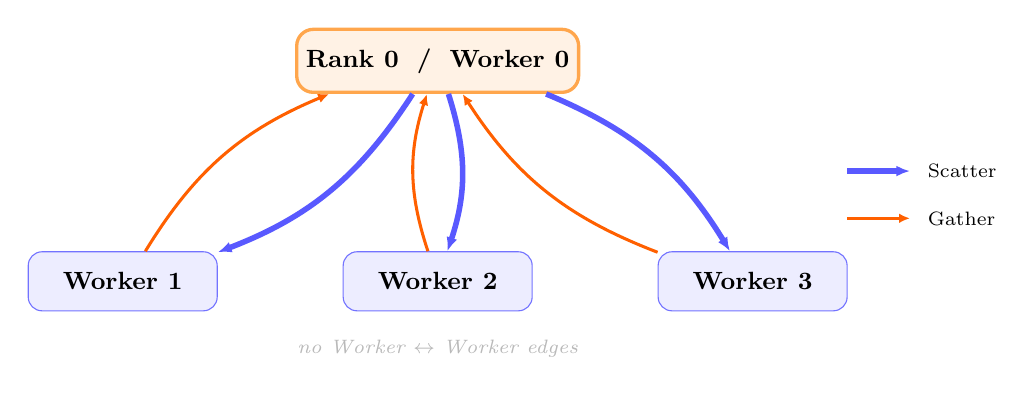
\begin{tikzpicture}[
  root/.style  = {draw=orange!70, fill=orange!10, rounded corners=6pt,
                  minimum width=3.0cm, minimum height=0.80cm,
                  font=\small\bfseries, line width=1.2pt},
  wnode/.style = {draw=blue!55, fill=blue!7, rounded corners=5pt,
                  minimum width=2.4cm, minimum height=0.75cm,
                  font=\small\bfseries},
  sarr/.style  = {-{Latex[length=5pt,width=4pt]}, line width=2.0pt,
                  blue!65},
  garr/.style  = {-{Latex[length=4pt,width=3.5pt]}, line width=1.1pt,
                  orange!75!red},
  lbl/.style   = {font=\scriptsize, fill=white, inner sep=1pt},
]

\node[root]  (r0) at ( 0,   2.8) {Rank 0 \;/\; Worker 0};
\node[wnode] (r1) at (-4.0, 0)   {Worker 1};
\node[wnode] (r2) at ( 0,   0)   {Worker 2};
\node[wnode] (r3) at ( 4.0, 0)   {Worker 3};

\draw[sarr] (r0) to[bend left=18] (r1);
\draw[sarr] (r0) to[bend left=18] (r2);
\draw[sarr] (r0) to[bend left=18] (r3);

\draw[garr] (r1) to[bend left=18] (r0);
\draw[garr] (r2) to[bend left=18] (r0);
\draw[garr] (r3) to[bend left=18] (r0);

\node[font=\scriptsize\itshape, gray!55]
  at (0, -0.85) {no Worker $\leftrightarrow$ Worker edges};

%% Legend
\draw[sarr] (5.2, 1.4) -- (6.0, 1.4);
\node[font=\scriptsize, anchor=west] at (6.1, 1.4) {Scatter};
\draw[garr] (5.2, 0.8) -- (6.0, 0.8);
\node[font=\scriptsize, anchor=west] at (6.1, 0.8) {Gather};

\end{tikzpicture}
\caption{Task Interaction Graph for $p=4$. The star topology
  has $O(p)$ edges total.}
\label{fig:tig}
\end{figure}

\textbf{Granularity lower bound from the TIG.}
The TIG edges carry quantifiable communication volumes and therefore establish
a lower bound on useful task granularity. A task is worth executing
independently only if its computation time $T_\text{comp}$ exceeds the edge
communication cost $T_\text{comm}$; below that threshold the worker spends
more time transferring data than computing, and agglomeration is the correct
response (Foster's \emph{Agglomerate} phase).

For this implementation the dominant edge cost per rank is the scatter message:
$N_\text{test}/p \times F \times 8~\text{bytes}
 = 5{,}000 \times 20 \times 8 = 800$~KB at $p=4$.
At a representative 1\,Gb/s cluster interconnect ($\approx$125\,MB/s), this
transfers in $\approx$6.4~ms. The measured compute time per rank is
$\approx$7.2~s at $p=4$, $t=1$, giving a granularity ratio of
$T_\text{comp}/T_\text{comm} \approx 7200\,\text{ms}/6.4\,\text{ms}
\approx 1{,}100$.
The computation is more than three orders of magnitude larger than the
communication cost; the current decomposition is safely \emph{coarse-grained}.
This ratio also defines the granularity lower bound: tasks should contain at
least $\lceil 6.4\,\text{ms} / 1.44\,\text{ms per sample} \rceil \approx 5$
samples to break even on such a network.
The current granularity (5{,}000 samples/rank) is approximately 1{,}000$\times$
above this floor, confirming that further decomposition down to tens of samples
per rank would remain communication-efficient.

% ─────────────────────────────────────────────────────────────────────────────
\section{Communication}
\label{sec:communication}
% ─────────────────────────────────────────────────────────────────────────────

Three MPI patterns are used, each for a different purpose.

\subsection{MPI\_Scatter for the Input Distribution}

Before the timed loop, rank~0 splits and sends the test data:

\begin{lstlisting}[language=C++]
MPI_Scatter(X_test_all.data(),
            local_n_test * N_FEATURES, MPI_DOUBLE,
            X_test_local.data(),
            local_n_test * N_FEATURES, MPI_DOUBLE,
            0, MPI_COMM_WORLD);
\end{lstlisting}

\texttt{MPI\_Scatter} is a one-to-all collective: rank~0 splits a contiguous
buffer into equal chunks and sends one to each rank. The test set is trimmed
to a multiple of $p$ before scattering. This call is \emph{outside} the
timing loop. At $p=4$, each scatter message carries
$5{,}000 \times 20 \times 8 = 800$~KB; total scatter volume is 3.2~MB,
transferred once before timing begins.

\subsection{MPI\_Isend / MPI\_Irecv + MPI\_Waitall for the Result Gathering}

After inference, predictions are gathered at rank~0 using non-blocking
point-to-point operations:

\begin{lstlisting}[language=C++]
if (rank == 0) {
    std::copy(local_preds.begin(), local_preds.end(),
              global_preds.begin());
    std::vector<MPI_Request> reqs(size - 1);
    for (int r = 1; r < size; ++r)
        MPI_Irecv(global_preds.data() + r * local_n_test,
                  local_n_test, MPI_INT,
                  r, 0, MPI_COMM_WORLD, &reqs[r - 1]);
    MPI_Waitall((int)reqs.size(), reqs.data(), MPI_STATUSES_IGNORE);
} else {
    MPI_Request req;
    MPI_Isend(local_preds.data(), local_n_test,
              MPI_INT, 0, 0, MPI_COMM_WORLD, &req);
    MPI_Wait(&req, MPI_STATUS_IGNORE);
}
\end{lstlisting}

Rank~0 posts all receives at once, allowing multiple transfers to proceed
concurrently, then \texttt{MPI\_Waitall} blocks until all are done.
At $p=4$, each gather message is $5{,}000 \times 4 = 20$~KB; total gather
volume is 60~KB, negligible relative to the inference time.

\subsection{MPI\_Reduce for the Accuracy Check}

Each rank counts how many of its local predictions are correct.
A single \texttt{MPI\_Reduce} sums the counts at rank~0:

\begin{lstlisting}[language=C++]
MPI_Reduce(&local_correct, &global_correct, 1,
           MPI_LONG, MPI_SUM, 0, MPI_COMM_WORLD);
\end{lstlisting}

This is outside the timing loop and communicates one integer per rank,
instead of sending individual labels again.


% ─────────────────────────────────────────────────────────────────────────────
\section{Agglomeration}
\label{sec:agglomeration}
% ─────────────────────────────────────────────────────────────────────────────

\subsection{Granularity}

At the finest level, each of the 20{,}000 test samples is an independent task.
One MPI rank per sample is impractical, the spawn and communication overhead
would dominate. Tasks are therefore agglomerated in two stages:

\begin{enumerate}
  \item \textbf{MPI level.} All $N_\text{test}/p$ samples for a rank are
        processed as one block. MPI message count is $O(p)$, independent
        of $N_\text{test}$.
  \item \textbf{OpenMP level.} Within each rank, the loop over local samples
        is parallelised with a single \texttt{\#pragma omp parallel for}.
        This gives exactly \emph{one} fork/join per run --- not one per sample.
        A single fork/join on Linux costs $\approx$2--5~$\mu$s; amortised
        over ${\sim}5{,}000$ samples per rank this is $<$0.1\% of a 7~s run,
        versus ${\sim}10$~ms if forked per sample.
\end{enumerate}

\subsection{KNN Buffer Strategy}

Each OpenMP thread gets its own distance buffer and index buffer (both of
length 50{,}000), allocated once before the timing loop and indexed by
\texttt{omp\_get\_thread\_num()}. This eliminates up to 100{,}000 heap
allocations per run and avoids false sharing between threads. Cache lines
on this platform are 64~bytes (8 doubles); because each thread's buffers
are independent heap allocations their first elements land on different
cache lines, so threads never invalidate each other's L1/L2 entries.

\subsection{KNN Cache Tiling}

The KNN kernel uses a two-level blocking scheme (\texttt{TILE\_Q}=4,
\texttt{TILE\_T}=512) to reduce L3 pressure. Instead of computing all
distances for one query before moving to the next, it processes
\texttt{TILE\_Q}=4 queries simultaneously against a tile of
\texttt{TILE\_T}=512 training rows ($512 \times 20 \times 8 = 80$~KB,
fitting comfortably in the 256~KB L2 cache). Each tile is loaded once
from L3/DRAM and reused for all 4 queries before eviction, cutting the
effective L3 bandwidth demand by ${\approx}$\texttt{TILE\_Q}$\times$.
This is why the measured throughput is significantly higher than a
naïve per-query implementation would achieve;
Figure~\ref{fig:cache_tiling} contrasts the two memory-access patterns.
Each rank loads \texttt{X\_train} independently from disk, so all $p$ ranks
stream their own copy without contending for the same cache lines across
processes.

\begin{figure}[H]
\centering
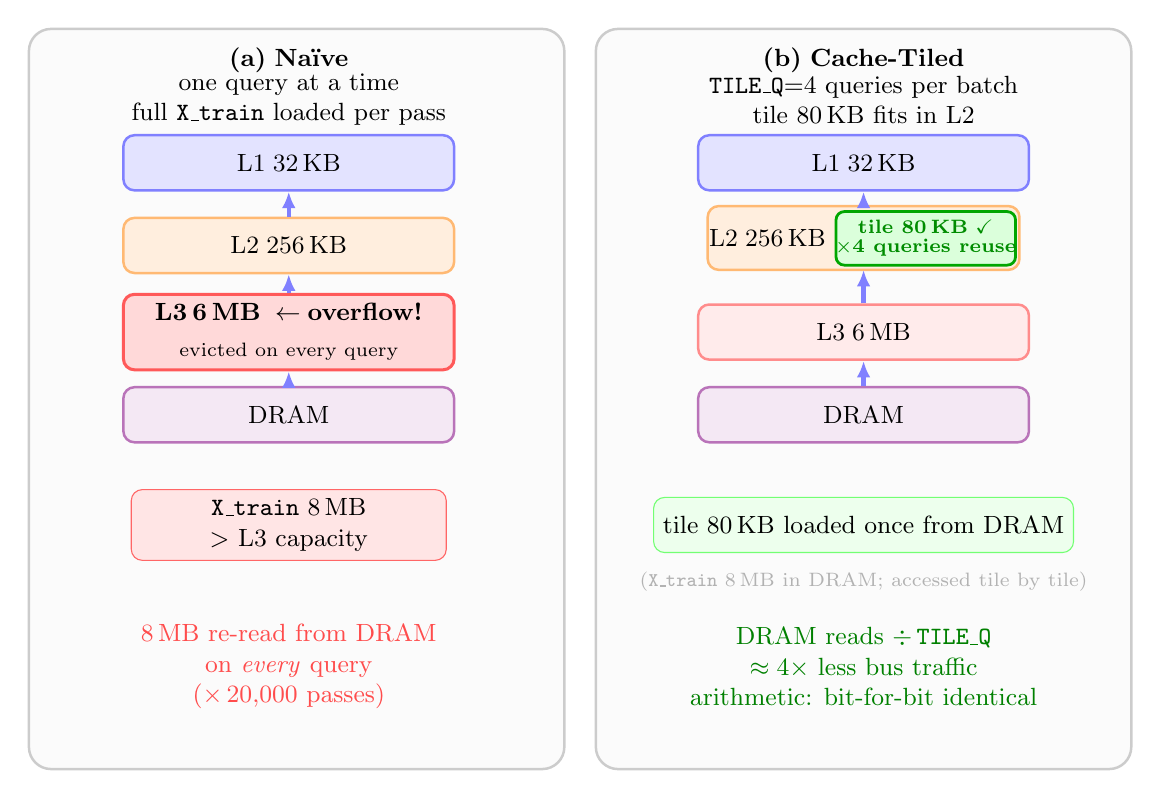
\begin{tikzpicture}[
  mbox/.style  = {rounded corners=4pt, minimum width=4.2cm,
                  minimum height=0.70cm, font=\small,
                  line width=0.9pt, text centered},
  darr/.style  = {-{Latex[length=6pt,width=5pt]}, line width=1.5pt},
  bg/.style    = {draw=gray!40, fill=gray!3, rounded corners=8pt,
                  line width=0.9pt},
]

%% ── (a) Naïve ───────────────────────────────────────────────────────────────
\draw[bg] (-6.3,-4.0) rectangle (0.5, 5.4);
\node[font=\small\bfseries]      at (-3.0, 5.00) {(a)\;Naïve};
\node[font=\small, align=center] at (-3.0, 4.50)
  {one query at a time\\full \texttt{X\_train} loaded per pass};

\node[mbox, draw=blue!50,   fill=blue!11]   (L1a) at (-3.0, 3.70) {L1\;32\,KB};
\node[mbox, draw=orange!55, fill=orange!13] (L2a) at (-3.0, 2.65) {L2\;256\,KB};

\node[mbox, draw=red!65, fill=red!15, line width=1.1pt,
      minimum height=0.92cm, align=center] (L3a) at (-3.0, 1.55)
  {\textbf{L3\,6\,MB}\;\;$\leftarrow$\;\textbf{overflow!}\\[2pt]
   {\scriptsize evicted on every query}};

\node[mbox, draw=violet!55, fill=violet!9] (DRa) at (-3.0, 0.50) {DRAM};

\draw[darr, blue!50] (DRa.north) -- (L3a.south);
\draw[darr, blue!50] (L3a.north) -- (L2a.south);
\draw[darr, blue!50] (L2a.north) -- (L1a.south);

\node[draw=red!60, fill=red!10, rounded corners=4pt,
      minimum width=4.0cm, minimum height=0.84cm,
      font=\small, align=center] at (-3.0,-0.90)
  {\texttt{X\_train} 8\,MB\\$>$ L3 capacity};

\node[font=\small, red!70, align=center] at (-3.0,-2.70)
  {8\,MB re-read from DRAM\\
   on \emph{every} query\\
   $(\times\,20{,}000$ passes$)$};

%% ── (b) Cache-Tiled ─────────────────────────────────────────────────────────
\draw[bg] (0.9,-4.0) rectangle (7.7, 5.4);
\node[font=\small\bfseries]      at (4.3, 5.00) {(b)\;Cache-Tiled};
\node[font=\small, align=center] at (4.3, 4.50)
  {\texttt{TILE\_Q}=4 queries per batch\\tile 80\,KB fits in L2};

\node[mbox, draw=blue!50, fill=blue!11] (L1b) at (4.3, 3.70) {L1\;32\,KB};

\draw[draw=orange!55, fill=orange!13, rounded corners=4pt, line width=0.9pt]
  (2.32, 2.34) rectangle (6.28, 3.15);
\node[font=\small] at (3.08, 2.74) {L2\;256\,KB};

\draw[draw=green!65!black, fill=green!14, rounded corners=3pt, line width=1.0pt]
  (3.95, 2.40) rectangle (6.23, 3.08);
\node[font=\scriptsize\bfseries, green!55!black, align=center] at (5.09, 2.74)
  {tile 80\,KB\;\checkmark\\[-1pt]$\times$4 queries reuse};

\node[mbox, draw=red!45,    fill=red!8]    (L3b) at (4.3, 1.55) {L3\;6\,MB};
\node[mbox, draw=violet!55, fill=violet!9] (DRb) at (4.3, 0.50) {DRAM};

\draw[darr, blue!50] (DRb.north) -- (L3b.south);
\draw[darr, blue!50] (L3b.north) -- (4.3, 2.34);
\draw[darr, blue!50] (4.3, 3.15) -- (L1b.south);

\node[draw=green!55, fill=green!7, rounded corners=4pt,
      minimum width=4.0cm, minimum height=0.70cm,
      font=\small, align=center] at (4.3,-0.90)
  {tile 80\,KB loaded once from DRAM};
\node[font=\scriptsize, gray!60, align=center] at (4.3,-1.62)
  {(\texttt{X\_train} 8\,MB in DRAM; accessed tile by tile)};

\node[font=\small, green!50!black, align=center] at (4.3,-2.70)
  {DRAM reads $\div$\,\texttt{TILE\_Q}\\
   $\approx 4\times$ less bus traffic\\
   arithmetic: bit-for-bit identical};

\end{tikzpicture}
\caption{Cache-tiling principle for the KNN distance kernel.
  \emph{(a)} Naïve: the full $50{,}000 \times 20 \times 8 = 8$\,MB
  training set overflows the 6\,MB L3 and is re-read from DRAM on every
  query ($\times\,N_\text{test} = 20{,}000$ passes total).
  \emph{(b)} Tiled: a tile of \texttt{TILE\_T}=512 training rows
  ($512\times20\times8 = 80$\,KB) fits inside the 256\,KB L2 cache.
  The tile is loaded once and reused for all \texttt{TILE\_Q}=4 queries
  in the current batch before eviction, reducing effective DRAM bandwidth
  by $\approx\texttt{TILE\_Q}\times$.}
\label{fig:cache_tiling}
\end{figure}

% ─────────────────────────────────────────────────────────────────────────────
\section{Mapping}
\label{sec:mapping}
% ─────────────────────────────────────────────────────────────────────────────

\subsection{Hardware Platform}
\label{sec:hw_platform}

The experiments run on an Intel Core i5-8350U with 4 physical cores and 8
logical threads (Hyper-Threading), under Ubuntu~22.04 / WSL2 on Windows~11.
This is a single-socket CPU; Non-Uniform Memory Access (NUMA) effects do
not apply.

Figure~\ref{fig:hw_arch} shows the memory hierarchy. The most important
detail is that the KNN working set ($50{,}000 \times 20 \times 8 = 8$~MB)
\textbf{exceeds the 6~MB L3 cache}. Every KNN call therefore reads from DRAM,
making the kernel memory-bandwidth-bound. This is the main reason speedup
does not scale linearly beyond 4 physical cores.

\begin{figure}[H]
\centering
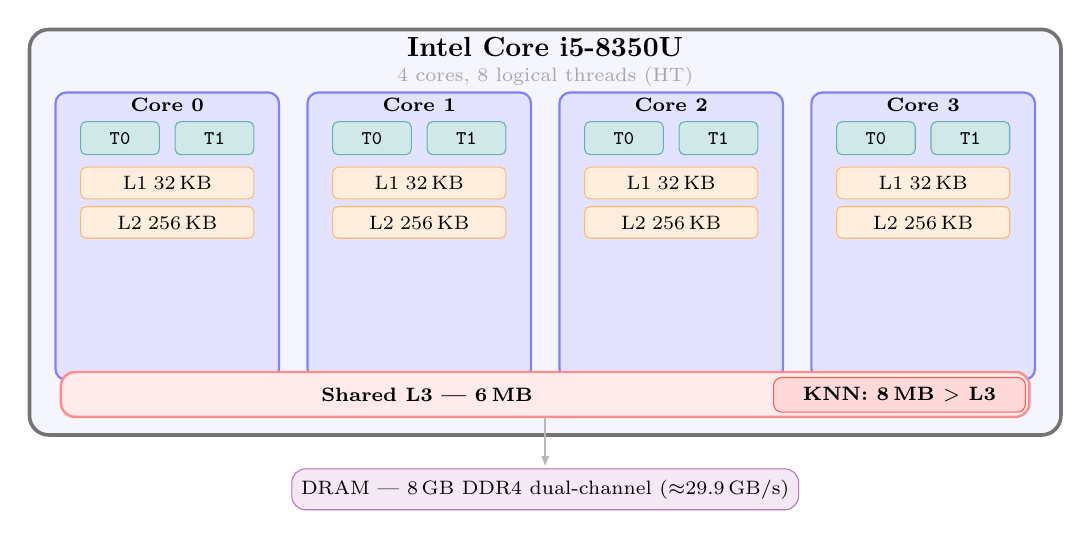
\begin{tikzpicture}[
  chip/.style    = {draw=black!55, fill=blue!4,   rounded corners=7pt, line width=1.3pt},
  cbox/.style    = {draw=blue!50,  fill=blue!11,  rounded corners=4pt, line width=0.8pt},
  htbox/.style   = {draw=teal!60,  fill=teal!18,  rounded corners=2pt,
                    minimum width=1.0cm, minimum height=0.42cm, font=\scriptsize\ttfamily},
  privbox/.style = {draw=orange!55,fill=orange!13,rounded corners=2pt,
                    minimum width=2.2cm, minimum height=0.40cm, font=\scriptsize},
  l3box/.style   = {draw=red!45,   fill=red!8,    rounded corners=5pt, line width=0.9pt},
  drambox/.style = {draw=violet!55,fill=violet!9, rounded corners=5pt,
                    minimum width=5.0cm, minimum height=0.52cm, font=\scriptsize},
  warn/.style    = {draw=red!65,   fill=red!15,   rounded corners=3pt,
                    minimum width=3.2cm, minimum height=0.44cm, font=\scriptsize\bfseries},
]

\draw[chip] (-6.55,-2.05) rectangle (6.55, 3.1);
\node[font=\bfseries\normalsize] at (0, 2.88) {Intel Core i5-8350U};
\node[font=\scriptsize, gray!70] at (0, 2.50)
  {4 cores, 8 logical threads (HT)};

\foreach \idx/\cx in {0/-4.8, 1/-1.6, 2/1.6, 3/4.8}{
  \draw[cbox] (\cx-1.42, -1.35) rectangle (\cx+1.42, 2.30);
  \node[font=\scriptsize\bfseries] at (\cx, 2.14) {Core \idx};
  \node[htbox] at (\cx-0.60, 1.72) {T0};
  \node[htbox] at (\cx+0.60, 1.72) {T1};
  \node[privbox] at (\cx, 1.15) {L1\;32\,KB};
  \node[privbox] at (\cx, 0.65) {L2\;256\,KB};
}

\draw[l3box] (-6.15,-1.25) rectangle (6.15,-1.82);
\node[font=\scriptsize\bfseries] at (-1.5,-1.54) {Shared L3 --- 6\,MB};
\node[warn] at (4.5,-1.54) {KNN: 8\,MB $>$ L3};

\draw[-{Latex[length=4pt]}, gray!55, line width=0.9pt] (0,-1.82) -- (0,-2.46);
\node[drambox] at (0,-2.74)
  {DRAM --- 8\,GB DDR4 dual-channel ($\approx$29.9\,GB/s)};

\end{tikzpicture}
\caption{Memory hierarchy of the test platform. L1/L2 caches are private
  per core; the 6\,MB L3 is shared. The KNN training data (8\,MB) exceeds
  the L3, forcing all threads to stream from DRAM and saturating the shared
  memory bus as core count grows.}
\label{fig:hw_arch}
\end{figure}

\subsection{Load Balancing and Minimal Idling}

The mapping strategy is designed to minimise idle time through static load
balancing at both parallelism levels.

\textbf{MPI level.}
\texttt{MPI\_Scatter} distributes the test set in equal slices of
$N_\text{test}/p$ samples to each rank. Equal distribution is valid here
because the per-sample cost is \emph{homogeneous}: every test sample searches
the same 50{,}000-point training set, so an equal sample count implies equal
compute time and zero rank-level load imbalance.

\textbf{OpenMP level.}
Within each rank, \texttt{schedule(static)} divides the local
$N_\text{test}/p$ samples into $t$ equal-sized contiguous blocks.
Contiguous assignment also preserves spatial locality (hardware prefetch
streams step through \texttt{X\_test\_local} in order). A dynamic schedule
would interleave accesses across threads and break the sequential stride;
it would only be preferable if samples had variable cost, which they do not.

\textbf{Residual idle time.}
The only unavoidable idle periods are: (i)~rank~0 coordinates the gather and
reduce phases while workers wait; (ii)~the sample-count trimming described in
Section~\ref{sec:decomposition} introduces a negligible $< 0.01\%$ workload
imbalance. All other idle time is eliminated by the static equal-partition
strategy.

\subsection{Configurations Tested}

No explicit CPU affinity is set; the OS scheduler assigns cores.
Without pinning, the two OpenMP threads within a rank may be scheduled on
different physical cores rather than on the physical/HT sibling pair assumed
in Figure~\ref{fig:mapping}. If so, per-rank memory pressure decreases
(each thread gets its own L2), but the co-location model would not hold.
The configurations tested are listed below, where $p$ = MPI ranks
and $t$ = OpenMP threads per rank. All configurations use the same
hybrid binary \texttt{inference\_dist\_knn}; $t=1$ simply means
OpenMP parallelism is inactive within each rank.

\begin{table}[H]
  \centering
  \caption{Tested configurations. Each MPI rank maps to one physical core;
           $t=2$ adds the Hyper-Threading sibling of that core.}
  \begin{tabular}{cccl}
    \toprule
    $p$ & $t$ & $p \cdot t$ & Notes \\
    \midrule
    1 & 1 & 1 & parallel baseline ($T_1$) \\
    1 & 2 & 2 & OpenMP-level parallelism only \\
    2 & 1 & 2 & 1 thread/rank, 2 physical cores \\
    2 & 2 & 4 & hybrid, 2 cores + HT siblings \\
    3 & 1 & 3 & 1 thread/rank, 3 physical cores \\
    4 & 1 & 4 & 1 thread/rank, all 4 physical cores \\
    3 & 2 & 6 & hybrid, 3 cores + HT siblings \\
    4 & 2 & 8 & hybrid, all 4 cores + HT siblings \\
    \bottomrule
  \end{tabular}
\end{table}

Figure~\ref{fig:mapping} shows how the two $p=4$ configurations
map onto the physical hardware.

\begin{figure}[H]
\centering
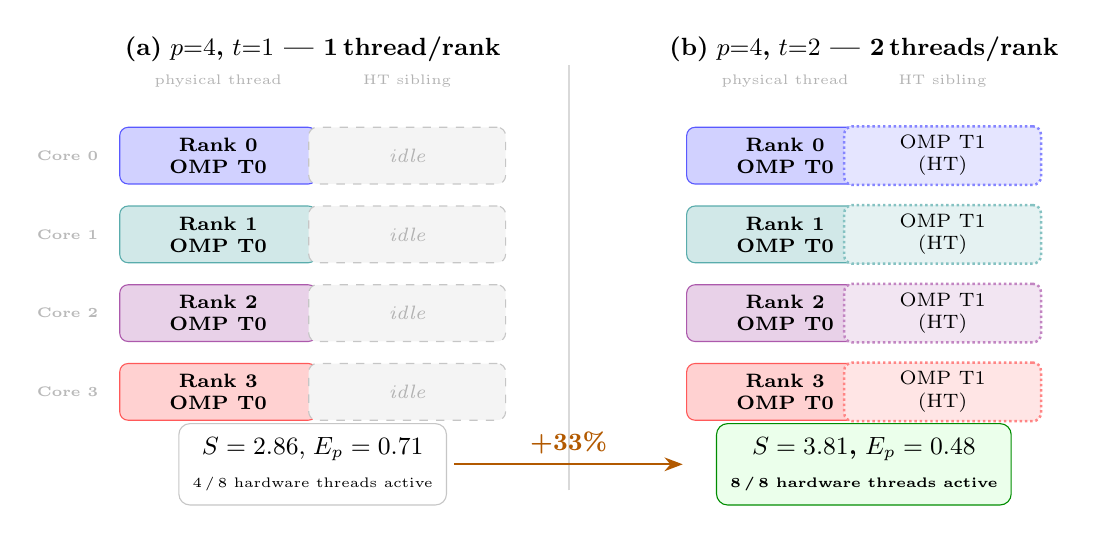
\begin{tikzpicture}[
  act/.style   = {draw=#1!65, fill=#1!18, rounded corners=3pt,
                  minimum width=2.5cm, minimum height=0.72cm,
                  font=\scriptsize\bfseries, align=center},
  htact/.style = {draw=#1!48, fill=#1!10, rounded corners=3pt,
                  minimum width=2.5cm, minimum height=0.72cm,
                  font=\scriptsize, align=center,
                  densely dotted, line width=0.9pt},
  idle/.style  = {draw=gray!45, fill=gray!9, rounded corners=3pt,
                  minimum width=2.5cm, minimum height=0.72cm,
                  font=\scriptsize\itshape, align=center, dashed,
                  text=gray!60},
]

%% column titles
\node[font=\small\bfseries] at (-2.95, 4.65)
  {(a)\;$p{=}4$,\;$t{=}1$ --- 1\,thread/rank};
\node[font=\small\bfseries] at ( 4.05, 4.65)
  {(b)\;$p{=}4$,\;$t{=}2$ --- 2\,threads/rank};

%% sub-column headers
\node[font=\tiny, gray!60] at (-4.15, 4.25) {physical thread};
\node[font=\tiny, gray!60] at (-1.75, 4.25) {HT sibling};
\node[font=\tiny, gray!60] at ( 3.05, 4.25) {physical thread};
\node[font=\tiny, gray!60] at ( 5.05, 4.25) {HT sibling};

%% one row per physical core
\foreach \i/\col in {0/blue, 1/teal, 2/violet, 3/red}{
  \pgfmathsetmacro{\y}{3.30 - \i * 1.0}
  \node[font=\tiny\bfseries, gray!55, anchor=east] at (-5.55, \y) {Core \i};
  \node[act=\col]   at (-4.15, \y) {Rank \i\\OMP T0};
  \node[idle]       at (-1.75, \y) {idle};
  \node[act=\col]   at ( 3.05, \y) {Rank \i\\OMP T0};
  \node[htact=\col] at ( 5.05, \y) {OMP T1\\(HT)};
}

%% vertical divider between the two configurations
\draw[gray!30, line width=0.7pt] (0.30, -0.95) -- (0.30, 4.45);

%% speedup summary
\node[draw=gray!45, fill=white, rounded corners=4pt, font=\small,
      align=center, inner sep=5pt] at (-2.95, -0.62)
  {$S=2.86$,\;$E_p=0.71$\\[1pt]{\tiny 4\,/\,8 hardware threads active}};

\node[draw=green!55!black, fill=green!8, rounded corners=4pt,
      font=\small\bfseries, align=center, inner sep=5pt] at (4.05, -0.62)
  {$S=3.81$,\;$E_p=0.48$\\[1pt]{\tiny 8\,/\,8 hardware threads active}};

%% gain annotation
\draw[-{Stealth}, thick, orange!70!black]
  (-1.15, -0.62) -- (1.75, -0.62)
  node[midway, above, font=\small\bfseries, orange!70!black] {+33\%};

\end{tikzpicture}
\caption{Hardware mapping for $p{=}4$: each row is one physical core of the
  i5-8350U; each column pair shows the physical thread (solid border) and its
  Hyper-Threading sibling (dotted or dashed).
  (a)~$t{=}1$: the HT slot in every core is idle, leaving half the chip's
  thread capacity unused. (b)~$t{=}2$: a second OpenMP thread per rank fills
  those slots, raising speedup from $S=2.86$ to $S=3.81$ (+33\%). Efficiency
  still drops because all four ranks share one DRAM bus, saturating memory
  bandwidth even with threads added.}
\label{fig:mapping}
\end{figure}

% ─────────────────────────────────────────────────────────────────────────────
\section{Performance Evaluation}
\label{sec:perf}
% ─────────────────────────────────────────────────────────────────────────────

\subsection{Setup}

\begin{itemize}
  \item \textbf{Machine:} Intel Core i5-8350U, 4 physical cores, 8 logical
        threads, 6~MB L3, 15~W TDP, Ubuntu~22.04 / WSL2.
  \item \textbf{Compiler:} \texttt{mpic++}, optimisation \texttt{-O2} for
        all binaries (including the sequential baseline).
  \item \textbf{Measurement:} 3 runs per configuration; median time reported.
        Min and max values are also recorded to show variance.
        Each run starts with \texttt{MPI\_Barrier} to synchronise all ranks
        before \texttt{MPI\_Wtime()} begins timing.
  \item \textbf{Baseline:} $T_1 = 20.60$~s, taken from the hybrid binary
        (\texttt{inference\_dist\_knn}) at $p=1$, $t=1$, cold page cache.
        Using the same binary as the baseline ensures a fair apples-to-apples
        comparison: every parallel configuration is measured against the
        identical code path with parallelism inactive, not against a
        separately compiled sequential implementation that may have different
        data-loading paths and no MPI overhead.
  \item \textbf{Metrics:} speedup $S_p = T_1 / T_p$; efficiency
        $E_p = S_p / (p \times t)$, where $p \times t$ is the total worker
        count (MPI ranks $\times$ OpenMP threads per rank). For $t=1$
        configurations this reduces to $S_p / p$.
  \item \textbf{Cold page cache:} before every experiment the OS page cache
        was flushed (\texttt{sync \&\& echo 3 > /proc/sys/vm/drop\_caches})
        to ensure consistent cold-start DRAM access patterns. Without this
        step the kernel retains recently accessed file pages in RAM, so a
        second run of the same configuration reads the training set from
        the page cache rather than from disk, and appears faster than it
        truly is. Production inference workloads operate on data that is
        not pre-loaded; the cold-cache baseline accurately models that
        scenario and prevents warm-cache runs from inflating the measured
        speedup.
  \item \textbf{Note on WSL2 and single-machine MPI:} experiments run under
        a virtualisation layer. MPI ranks communicate via shared-memory IPC
        rather than a real network interconnect, so inter-rank communication
        cost is near-zero. On a real cluster with a network fabric, MPI
        communication overhead would be measurably larger, and efficiency
        at high $p$ would be lower. Absolute timings may also be affected
        by WSL2 scheduling overhead; relative scaling trends remain
        meaningful.
\end{itemize}

\subsection{Strong Scaling Results}

\begin{table}[H]
  \centering
  \caption{Strong scaling benchmark results. $T_1 = 20.60$~s
           (hybrid binary at $p=1$, $t=1$, cold page cache).
           Speedup $S_p = T_1/T_p$;
           efficiency $E_p = S_p / (p \times t)$ uses total workers as the denominator.
           Min and max are from 3 repetitions.}
  \label{tab:results}
  \begin{tabular}{cccc cc c c}
    \toprule
    $p$ & $t$ & $p{\cdot}t$ & Min (s) & Time (s) & Max (s) & $S_p$ & $E_p$ \\
    \midrule
    1 & 1 & 1 & 19.37 & 20.60 & 21.24 & 1.000 & 1.000 \\
    1 & 2 & 2 & 10.41 & 11.27 & 11.64 & 1.829 & 0.914 \\
    2 & 1 & 2 & 10.99 & 11.10 & 12.59 & 1.855 & 0.928 \\
    2 & 2 & 4 &  6.85 &  7.93 &  8.20 & 2.597 & 0.649 \\
    3 & 1 & 3 &  8.12 &  8.28 &  8.75 & 2.490 & 0.830 \\
    3 & 2 & 6 &  5.75 &  7.05 &  7.33 & 2.922 & 0.487 \\
    4 & 1 & 4 &  6.91 &  7.21 &  7.35 & 2.857 & 0.714 \\
    4 & 2 & 8 &  5.37 &  5.40 &  5.56 & \textbf{3.812} & 0.477 \\
    \bottomrule
  \end{tabular}
\end{table}

\begin{figure}[H]
  \centering
  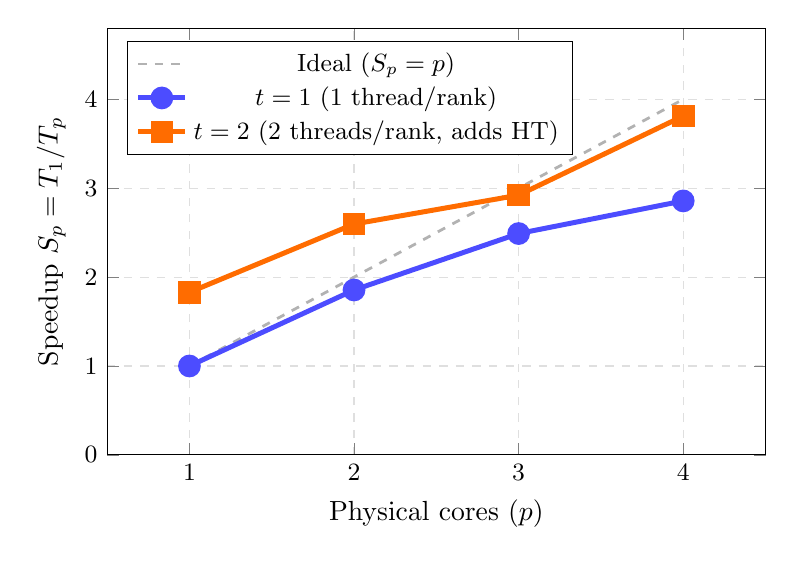
\begin{tikzpicture}
    \begin{axis}[
      width=0.82\textwidth, height=7cm,
      xlabel={Physical cores ($p$)},
      ylabel={Speedup $S_p = T_1 / T_p$},
      xmin=0.5, xmax=4.5, ymin=0, ymax=4.8,
      xtick={1,2,3,4}, ytick={0,1,2,3,4},
      ymajorgrids=true, xmajorgrids=true,
      grid style={dashed, gray!25},
      legend pos=north west, legend style={font=\small},
      tick label style={font=\small},
    ]
    \addplot[color=gray!60, dashed, line width=1.0pt, mark=none]
      coordinates {(1,1)(2,2)(3,3)(4,4)};
    \addlegendentry{Ideal ($S_p = p$)}

    \addplot[color=blue!70, solid, line width=1.8pt, mark=*, mark size=3.2pt]
      coordinates {(1,1.000)(2,1.855)(3,2.490)(4,2.857)};
    \addlegendentry{$t=1$ (1 thread/rank)}

    \addplot[color=orange!85!red, solid, line width=1.8pt,
             mark=square*, mark size=3.2pt]
      coordinates {(1,1.829)(2,2.597)(3,2.922)(4,3.812)};
    \addlegendentry{$t=2$ (2 threads/rank, adds HT)}

    \end{axis}
  \end{tikzpicture}
  \caption{Strong scaling speedup vs.\ physical cores $p$. Both series grow
    monotonically but sub-linearly. The $t=2$ series adds one HT thread per
    rank and is consistently faster; the gap between the two series narrows
    between $p=3$ and $p=4$, but the $t=2$ curve recovers to a best result
    of $3.81\times$ at $p=4$. Exact values are in Table~\ref{tab:results}.}
  \label{fig:speedup_line}
\end{figure}

\begin{figure}[H]
  \centering
  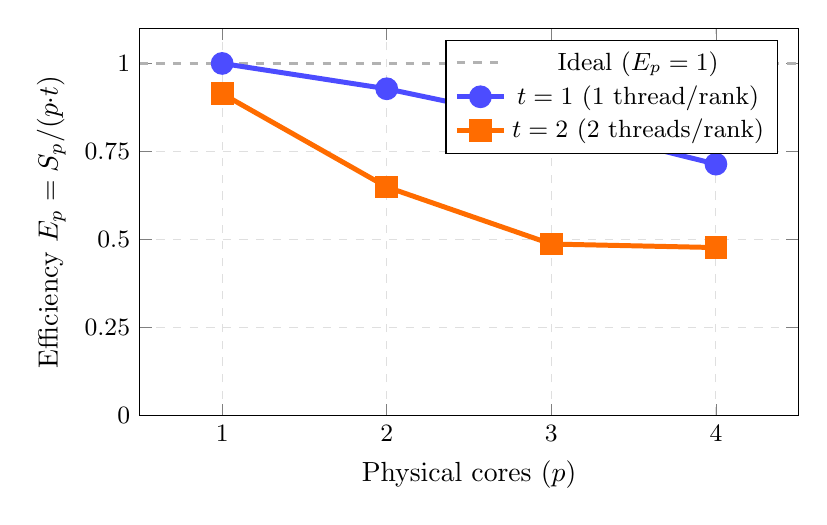
\begin{tikzpicture}
    \begin{axis}[
      width=0.82\textwidth, height=6.5cm,
      xlabel={Physical cores ($p$)},
      ylabel={Efficiency $E_p = S_p / (p{\cdot}t)$},
      xmin=0.5, xmax=4.5, ymin=0, ymax=1.1,
      xtick={1,2,3,4}, ytick={0,0.25,0.5,0.75,1.0},
      ymajorgrids=true, xmajorgrids=true,
      grid style={dashed, gray!25},
      legend pos=north east, legend style={font=\small},
      tick label style={font=\small},
    ]
    \addplot[color=gray!60, dashed, line width=1.0pt, mark=none]
      coordinates {(0.5,1.0)(4.5,1.0)};
    \addlegendentry{Ideal ($E_p = 1$)}

    \addplot[color=blue!70, solid, line width=1.8pt, mark=*, mark size=3.2pt]
      coordinates {(1,1.000)(2,0.928)(3,0.830)(4,0.714)};
    \addlegendentry{$t=1$ (1 thread/rank)}

    \addplot[color=orange!85!red, solid, line width=1.8pt,
             mark=square*, mark size=3.2pt]
      coordinates {(1,0.914)(2,0.649)(3,0.487)(4,0.477)};
    \addlegendentry{$t=2$ (2 threads/rank)}

    \end{axis}
  \end{tikzpicture}
  \caption{Efficiency $E_p = S_p/(p{\cdot}t)$ vs.\ physical cores. The $t=1$ series
    declines monotonically from $E_p=0.928$ at $p=2$ to $0.714$ at $p=4$,
    reflecting growing memory-bandwidth contention as more ranks stream
    \texttt{X\_train} concurrently. The $t=2$ series starts at $E_p=0.914$
    for $p=1$ (two threads, one rank) and converges toward the $t=1$ curve
    as $p$ grows and the shared DRAM bus becomes the common bottleneck.}
  \label{fig:efficiency}
\end{figure}

\subsection{Strong Scaling Analysis}
\label{sec:analysis_strong}

\textbf{Choice of baseline.}
The parallel baseline $T_1 = 20.60$~s is taken from the hybrid binary at
$p=1$, $t=1$. A separately compiled sequential binary
(\texttt{inference\_seq}) runs in 20.04~s, marginally faster because it
carries no MPI initialisation overhead. Using the same binary as the baseline
is the methodologically correct choice: every parallel row in
Table~\ref{tab:results} is measured against the identical code path, making
the comparison fair. The 3\% gap between the two binaries ($\approx$0.6~s) is
the fixed cost of the MPI framework at a single rank.

\textbf{Single-threaded baseline ($t=1$).}
At $p=2$ the $t=1$ configuration achieves $S=1.855$, $E_p=0.928$ ---
near-ideal utilisation of two independent cores. Efficiency declines steadily
to $E_p=0.714$ at $p=4$ as all four cores concurrently stream their own
8~MB copy of \texttt{X\_train} from DRAM, progressively saturating the
memory bus.

\textbf{HT contribution ($t=2$).}
Adding one HT thread per rank raises speedup at every physical core count:
\begin{itemize}
  \item $p=1$: $S$ rises from 1.000 to 1.829 (+83\%). A single HT thread
        provides substantial throughput because one thread can use execution
        units while the other stalls on DRAM loads.
  \item $p=2$: $S$ rises from 1.855 to 2.597 (+40\%).
  \item $p=3$: $S$ rises from 2.490 to 2.922 (+17\%). The HT gain diminishes
        as more threads compete for DRAM bandwidth.
  \item $p=4$: $S$ rises from 2.857 to \textbf{3.812} (+33\%). This is the
        \emph{best overall configuration}. All four physical cores are active
        and each HT sibling absorbs memory-latency stalls.
\end{itemize}

\textbf{MPI vs.\ OpenMP at equal worker count.}
At two total workers ($p=2,t=1$ vs.\ $p=1,t=2$): $S=1.855$ vs.\ $S=1.829$.
The two MPI ranks are marginally faster despite each holding an independent
copy of \texttt{X\_train} in DRAM: two separate processes have dedicated L1/L2
cache spaces, whereas two threads within one rank compete for the same caches.
At four total workers ($p=4,t=1$ vs.\ $p=2,t=2$): $S=2.857$ vs.\ $S=2.597$.
Four independent MPI ranks continue to outperform two hybrid ranks at the
same total worker count, confirming that the cache isolation of independent
processes is more beneficial than the shared-memory advantage of OpenMP at
this working-set size.

\textbf{Arithmetic intensity and the memory wall.}
Each distance computation in KNN performs approximately 40 floating-point
operations per training point (one subtraction and one multiply-accumulate
per feature, across 20 features), while reading 160 bytes (20
double-precision values), yielding an arithmetic intensity of
$40 / 160 = 0.25$~FLOP/byte. This figure covers the distance accumulation
loop only; \texttt{partial\_sort} and related sort infrastructure contribute
$\approx 2\%$ of runtime (Table~\ref{tab:gprof}) and raise the effective
operation count slightly, but the kernel remains firmly bandwidth-bound.
The DDR4-2133 dual-channel bus has a theoretical peak of $\approx 34$~GB/s;
at typical DRAM efficiency ($\approx$88\%) the achievable bandwidth is
$\approx 29.9$~GB/s, implying a throughput ceiling of
$29.9 \times 0.25 \approx 7.5$~GFLOP/s --- far below the CPU's compute
ceiling. The kernel is therefore \emph{bandwidth-bound by construction}.

\textbf{Amdahl's Law.}
The serial fraction is estimated from the $t=1$ result at $p=4$,
which is free from HT effects and directly tied to physical processors.
For $S_p = 2.857$ at $p = 4$:
\[
  f = \frac{1/S_p - 1/p}{1 - 1/p}
    = \frac{0.3500 - 0.250}{0.750}
    \approx 0.133
\]
The implied ceiling is $1/f \approx 7.5\times$ on infinite physical cores.
Because memory contention inflates $f$ beyond the true serial fraction,
this is a \emph{lower bound} on the ceiling: on a machine with dedicated
per-rank memory buses the effective $f$ would approach the NB+LR fraction
($\approx 0.02\%$), raising the ceiling well above $7.5\times$.
The gap between the measured $f=0.133$ and the profiled NB+LR cost is
explained by memory-bandwidth contention, which serialises parallel threads
through the shared DRAM bus and inflates the apparent serial fraction beyond
what static profiling captures.

\textbf{Scalability.}
Scalability is defined as the ratio $E(n_2)/E(n_1)$ of two efficiency values,
quantifying how well efficiency is retained as the worker count increases.
For the $t=1$ series (pure MPI scaling, free of HT effects):
\begin{itemize}
  \item $p=1 \to p=2$: $E=1.000 \to 0.928$,\quad
        retention $= 0.928/1.000 = 0.928$ ($92.8\%$).
  \item $p=2 \to p=3$: $E=0.928 \to 0.830$,\quad
        retention $= 0.830/0.928 = 0.895$ ($89.5\%$).
  \item $p=3 \to p=4$: $E=0.830 \to 0.714$,\quad
        retention $= 0.714/0.830 = 0.860$ ($86.0\%$).
\end{itemize}
Each step retains approximately 86--93\% of prior efficiency. The declining
trend is consistent with progressive memory-bandwidth saturation: as more
ranks concurrently stream independent 8\,MB copies of \texttt{X\_train},
the shared DRAM bus becomes increasingly contested and the marginal return of
each additional rank diminishes.

\subsection{Weak Scaling Results and Analysis}

Weak scaling fixes the \emph{work per rank} (1{,}000 test samples/rank) and
grows the total problem size with the number of ranks. Under ideal scaling,
time is constant and efficiency $\eta_w = T_1^\text{rank} / T_p^\text{rank} = 1$.

\begin{table}[H]
  \centering
  \caption{Weak scaling results ($t=1$ thread per rank). Work per rank fixed
           at 1{,}000 samples. Baseline $T_1 = 1.025$~s (p=1, cold cache).
           Efficiency $\eta_w = T_1 / T_p$ (ideal: 1.0);
           speedup $S_w = p \times \eta_w$ (total throughput vs.\ sequential).
           Min and max are from 3 repetitions.}
  \label{tab:weak}
  \begin{tabular}{cc c ccc cc}
    \toprule
    $p$ & Samples/rank & Total & Min (s) & Time (s) & Max (s) & $\eta_w$ & $S_w$ \\
    \midrule
    1 & 1{,}000 & 1{,}000 & 1.01 & 1.025 & 1.09 & 1.000 & 1.00 \\
    2 & 1{,}000 & 2{,}000 & 1.39 & 1.403 & 1.56 & 0.731 & 1.46 \\
    3 & 1{,}000 & 3{,}000 & 1.07 & 1.394 & 1.60 & 0.735 & 2.21 \\
    4 & 1{,}000 & 4{,}000 & 1.20 & 1.212 & 1.24 & 0.846 & 3.38 \\
    \bottomrule
  \end{tabular}
\end{table}

Weak scaling is measured with $t=1$ thread per rank, isolating the effect
of adding MPI processes while keeping per-rank compute constant.
The min/max columns reveal high variance at $p=3$ (1.07--1.60~s, a 50\%
spread), indicating significant OS scheduling noise at this small
problem size under WSL2.

\textbf{Comparison with strong scaling efficiency:}

\begin{table}[H]
  \centering
  \caption{Efficiency comparison between strong and weak scaling ($t=1$).}
  \begin{tabular}{c cc c}
    \toprule
    $p$ & Strong $E_p = S_p/p$ & Weak $\eta_w = T_1/T_p$ & Difference \\
    \midrule
    2 & 0.928 & 0.731 & $-$0.197 \\
    3 & 0.830 & 0.735 & $-$0.095 \\
    4 & 0.714 & 0.846 & $+$0.132 \\
    \bottomrule
  \end{tabular}
\end{table}

Unlike the classical expectation that weak scaling efficiency should be
\emph{higher} than strong scaling efficiency (because Amdahl's serial
fraction cancels out when work scales with $p$), weak scaling efficiency
falls \emph{below} strong scaling efficiency at $p=2$ and $p=3$.

The explanation lies in the nature of the fixed costs. In this implementation
the dominant fixed cost is loading the full training set: every rank, regardless
of how many test samples it processes, must read all 50{,}000 training points
($\approx$8~MB) from DRAM. With only 1{,}000 test samples per rank, the total
per-rank inference time is $\approx$1~s. MPI initialisation, scatter/gather
latency, and the cold-cache I/O hit on \texttt{X\_train} are absolute fixed
costs that do not shrink proportionally with the number of test samples.
At 1{,}000 samples/rank these overheads therefore consume a larger
\emph{fraction} of the $\approx$1~s run than of the $\approx$10~s strong
scaling run where each rank processes 10{,}000 samples. This depresses weak
scaling efficiency relative to strong scaling efficiency at small per-rank
workloads.

At $p=4$, weak efficiency (0.846) rises above strong efficiency (0.714).
This crossing should be treated with caution: the $p=3$ weak-scaling run
exhibited very high variance (min~1.07, max~1.60~s), making its median
unreliable. The $p=4$ run was stable (1.20--1.24~s). The apparent
recovery at $p=4$ is partly a measurement artifact of WSL2 scheduling noise
on a single machine rather than a genuine efficiency improvement.

% ─────────────────────────────────────────────────────────────────────────────
\section{Conclusion}
% ─────────────────────────────────────────────────────────────────────────────

A hybrid MPI + OpenMP parallel inference engine was designed, implemented,
and evaluated for a three-model soft-voting ensemble.
The architecture follows a deliberate two-level hybrid decomposition: MPI
distributes the test set across $p$ independent processes (coarse-grained,
distributed memory), while OpenMP subdivides each local slice among $t$
threads (fine-grained, shared memory). Total concurrency is $p \times t$.

The three MPI patterns required by the course specification are all present:
\texttt{MPI\_Scatter} for input distribution, non-blocking
\texttt{MPI\_Isend}/\texttt{MPI\_Irecv} + \texttt{MPI\_Waitall} for result
gathering, and \texttt{MPI\_Reduce} for accuracy validation.

Key results on the Intel Core i5-8350U ($T_1 = 20.60$~s, hybrid binary at
$p=1$, $t=1$, cold page cache):
\begin{itemize}
  \item Best speedup: $\mathbf{3.81\times}$ at $p=4$, $t=2$ (all physical
        cores + HT siblings).
  \item Best single-threaded efficiency: $E_p = 0.928$ at $p=2$, $t=1$.
  \item HT contribution at $p=1$: nearly doubles throughput ($S=1.83$)
        through latency hiding on DRAM-bound loads.
  \item At equal worker count ($p=2,t=1$ vs.\ $p=1,t=2$), MPI is marginally
        faster (1.855 vs.\ 1.829): two independent processes have dedicated
        cache space, outweighing the memory-duplication cost of OpenMP.
  \item Ensemble accuracy: \textbf{88.44\%} preserved across all
        configurations.
\end{itemize}

The dominant bottleneck is arithmetic intensity ($\approx 0.25$~FLOP/byte),
which makes the KNN kernel bandwidth-bound on the shared DRAM bus.
Amdahl's Law estimates a speedup ceiling of $\approx 7.5\times$ on infinite
physical cores, with an apparent serial fraction of $f \approx 0.133$
(above the $\approx$0.01\% NB+LR cost measured by the profiler; the gap is
attributable to memory contention serialising parallel threads through the
shared bus).

Weak scaling efficiency falls below strong scaling efficiency at $p=2$ and
$p=3$ because the fixed cost of loading \texttt{X\_train} (8~MB per rank)
dominates when per-rank work is only 1{,}000 test samples. This reveals a
limitation of the design: for small test sets the communication and I/O
overhead is disproportionately large relative to compute time.

All experiments ran on a single machine with MPI communication via
shared-memory IPC. On a real multi-node cluster, inter-node network
latency would add to the communication overhead, and the hybrid design
would become proportionally more advantageous: OpenMP exploits intra-node
shared memory (one \texttt{X\_train} copy per node instead of per rank),
while MPI handles inter-node distribution with $O(p_\text{nodes})$ messages,
directly alleviating the memory-bandwidth bottleneck observed here.

\addcontentsline{toc}{section}{References}

\begin{thebibliography}{9}

\bibitem{giacomazzi2006}
  P.~Giacomazzi et al.,
  ``A Parallel Implementation of the K Nearest Neighbours Classifier
    in Three Levels: Threads, MPI Processes and the Grid,''
  \textit{Parallel Computing}, 2006.

\bibitem{ignatij2022}
  I.~Ignatij,
  ``Parallel implementation of kNN using MPI,''
  GitHub repository, 2022.
  \url{https://github.com/ignatij/knn-mpi}

\bibitem{johnson2017faiss}
  J.~Johnson, M.~Douze, and H.~Jégou,
  ``Billion-scale similarity search with GPUs,''
  \textit{IEEE Transactions on Big Data}, vol.~7, no.~3, pp.~535--547, 2021.
  arXiv:1702.08734.

\end{thebibliography}
% ─────────────────────────────────────────────────────────────────────────────
\end{document}